\documentclass[a4paper]{article}
\pdfoutput=1
\usepackage[utf8]{inputenc}
\usepackage{tikz}
\usetikzlibrary{shapes,arrows,arrows.meta,matrix}
% \usetikzlibrary{snakes}
\usetikzlibrary{positioning,patterns}


\usetikzlibrary{external}
\tikzexternalize


\begin{document}


 \tikzset{
   treenode/.style = {align=center, inner sep=0pt, text centered},
   arn_n/.style = {treenode, circle,  draw=black, thick, text width=1.5em},% arbre rouge noir, noeud noir
   arn_r/.style = {treenode, circle, draw=red!80!, fill=red!20,text width=1.5em, very thick},% arbre rouge noir, noeud rouge
   arn_x/.style = {treenode, rectangle, draw=black, thick, minimum width=1.8em, minimum height=1.2em}% arbre rouge noir, nil
 }


  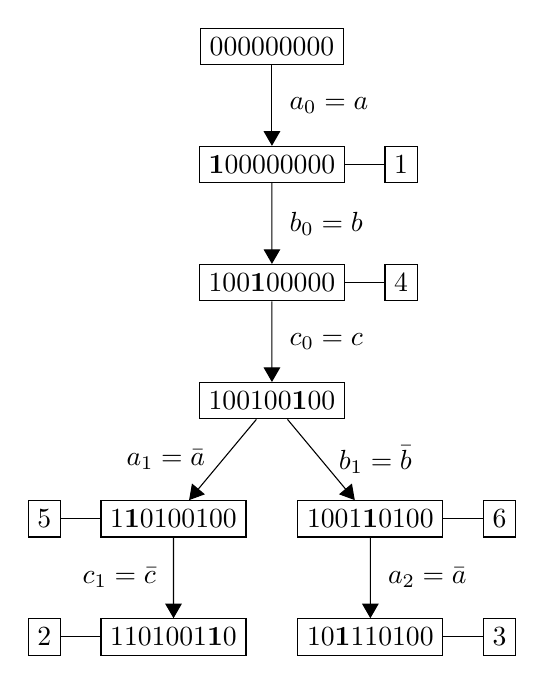
\begin{tikzpicture}[level distance=15mm,sibling distance=25mm,>=triangle 60,node distance=.5cm]
    \node[rectangle,draw]           (000) {000000000}
     child[->] {node[rectangle,draw]     (100) {\textbf{1}00000000}
		child {node[rectangle,draw]     (110) {100\textbf{1}00000}	    
     child {node[rectangle,draw]     (111) {100100\textbf{1}00}
   child {node[rectangle,draw]     (011) {1\textbf{1}0100100}
          child {node[rectangle,draw]  (010) {1101001\textbf{1}0}
            edge from parent node[left,xshift=-1mm] {$c_1=\bar c$}
          }
        edge from parent node[left,xshift=-1mm] {$a_1=\bar a$}
      }
      child {node[rectangle,draw]     (101) {1001\textbf{1}0100}
 	     child {node[rectangle,draw]     (001) {10\textbf{1}110100}
    	    edge from parent node[right,xshift=1mm] {$a_2=\bar a$}
      }
   	    edge from parent node[right,xshift=1mm] {$b_1=\bar b$} 
}
      edge from parent node[right,xshift=1mm] {$c_0=c$}
}
      edge from parent node[right,xshift=1mm] {$b_0=b$}    
}
      edge from parent node[right,xshift=1mm] {$a_0=a$}    
};

\node[rectangle,draw,right = of 100] (1) {$1$};
\node[rectangle,draw,right = of 110] (4) {$4$};
\node[rectangle,draw,left = of 011] (5) {$5$};
\node[rectangle,draw,left = of 010] (2) {$2$};
\node[rectangle,draw,right = of 101] (6) {$6$};
\node[rectangle,draw,right = of 001](3)  {$3$};

\draw (100) -- (1);
\draw (010) -- (2);
\draw (001) -- (3);
\draw (110) -- (4);
\draw (011) -- (5);
\draw (101) -- (6);

    %         \node[circle,draw]           (00000000) {}
    % child[->] {node[rectangle,draw]     (00010000) {$s_{4}$}
    %   child {node[rectangle,draw]     (00110000) {$s_{3}$}
    %     child {node[circle,draw]  (00111000) {}
    %       child {node[rectangle,draw]  (00111100) {$s_{2}$}
    %         edge from parent node[left] {$(c_{5},1)$}
    %       }
    %       child {node[rectangle,draw]     (01111000) {$s_{5}$}
    %         edge from parent node[right] {$(c_{1},1)$}
    %       }
    %       edge from parent node[left] {$(c_{4},1)$}
    %     }
    %     edge from parent node[left] {$(c_{2},1)$}
    %   }
    %   child {node[rectangle,draw]     (00010001) {$s_{1}$}
    %     edge from parent node[right] {$(c_{6},1)$}
    %   }
    %   edge from parent node[right] {$(c_{3},1)$}
    % };

    \end{tikzpicture}
\end{document}
